\documentclass[12pt]{article}
\usepackage[T2A]{fontenc}
\usepackage[utf8]{inputenc}
\usepackage{graphics}
\usepackage[english, russian]{babel}
\usepackage{csquotes}
\usepackage{graphicx}
\usepackage{amsmath}
\usepackage{longtable}
\usepackage[left=25mm, top=20mm, right=25mm, bottom=30mm,nohead,nofoot]{geometry}
\usepackage{verbatim}
\usepackage{hyperref}
\usepackage{amssymb,latexsym}  % Standard packages
\usepackage{MnSymbol}
\usepackage{mathrsfs}
\usepackage{amsthm}
\usepackage{indentfirst}
\usepackage[nottoc,numbib]{tocbibind}
\usepackage{float}

%******************************************************************
%******************************************************************

\setcounter{tocdepth}{4}
\graphicspath{ {./pic/} }

\renewcommand{\listoffigures}{\begingroup %добавляем номер в список иллюстраций
\tocsection
\tocfile{\listfigurename}{lof}
\endgroup}
\renewcommand{\listoftables}{\begingroup %добавляем номер в список таблиц
\tocsection
\tocfile{\listtablename}{lot}
\endgroup}

%******************************************************************
%******************************************************************

\begin{document}

\begin{titlepage}
	\center
		Санкт-Петербургский Политехнический 
		университет Петра Великого
		Институт прикладной математики и механики
		\\ \textbf{Кафедра «Прикладная математика»}

	\vfill ~
	\textbf{
		\\ \large ЛАБОРАТОРНАЯ РАБОТА №3
		\\	\normalsize	
			Боксплот Тьюки
	}
	\\	по дисциплине 
	\\	"Математическая статистика"

	\vfill 

	Выполнил студент гр. \textbf{33631/1} \\
	\textbf{Лансков.Н.В.} \\ 

\vfill

{\large}	Санкт-Петербург
\\ 2019
\end{titlepage}

%%%
% Table of conetnts 
%%%
% \settocdepth{chapter}
\tableofcontents
\newpage
\listoffigures{}
\newpage
\listoftables{}
\newpage
\pagebreak

% \setcounter{chapter}{1}

%%%
% Text
%%%
\section{Постановка задачи}
Для, приведённых ниже, пяти распределений сгенерировать выборки объёмом 20, 100, для каждой выборки построить боксплот Тьюки. Для каждого распределения определить процент выбросов экспериментально. Сгенерировать выборку, соответствующую распределению $1000$ раз и, вычислив средний процент, сравнить его с результатами, полученными теоретически.

Распределения:
\begin{enumerate}
\item Стандартное нормальное распределение
\item Стандартное распределение Коши
\item Распределение Лапласа с коэффициентом масштаба $\sqrt{2}$ и нулевым коэффициентом сдвига.
\item Равномерное распределение на отрезке $\left[-\sqrt{3}, \sqrt{3}\right]$
\item Распределение Пуассона со значением матожидания равным двум.
\end{enumerate}

\section{Теория}

Боксплот Тьюки - график, использующийся в описательной статистике, изображающий одномерное распределение вероятностей.

Такой вид диаграммы в удобной форме показывает медиану, нижний и верхний квартили, минимальное и максимальное значение выборки и выбросы.

\begin{enumerate}
\item Выборочная медиана \cite{med}:
\begin{equation}
med\; x = \begin{cases}
x_{k+1}, & n = 2k+1\\
\frac{1}{2}\left(x_k+x_{k+1}\right), & n = 2k
\end{cases} \hfill  \label{eqn:med}
\end{equation}

\item Квартиль \cite{quart}:
\begin{equation}
z_{[p]} = \begin{cases}
x_{np}, & np \in \mathbb{Z}\\
x_{[np]+1}, & np \notin \mathbb{Z}
\end{cases} \hfill  \label{eqn:quart}
\end{equation}
\end{enumerate}

Выбросом в статистике называют результат измерения, выделяющийся из общей выборки.


\section{Реализация}

Для генерации выборки был использован $Python\;3.7$: модуль $random$ библиотеки $numpy$ \cite{numpy}.

Боксплот Тьюки был построен средствами библиотеки matplotlib \cite{plotlib}.

Правая и левые границы:  $R- LQ - l(UQ - LQ),\;L = UQ -k(UQ - LQ),$ где $k$ обычно полагают равным $1.5$ 

\section{Результаты}

\begin{center}
\begin{figure}[H]
\caption{Boxplot нормальное распределение }
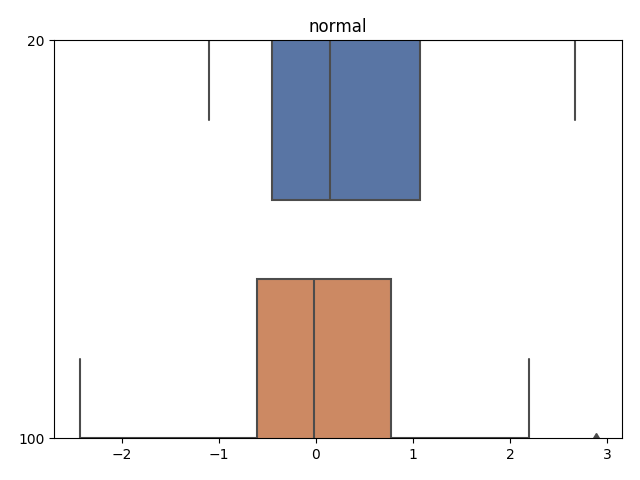
\includegraphics[width=\textwidth]{normal.png}
\end{figure}

\begin{figure}[H]
\caption{Boxplot стандартное распределение Лапласа }
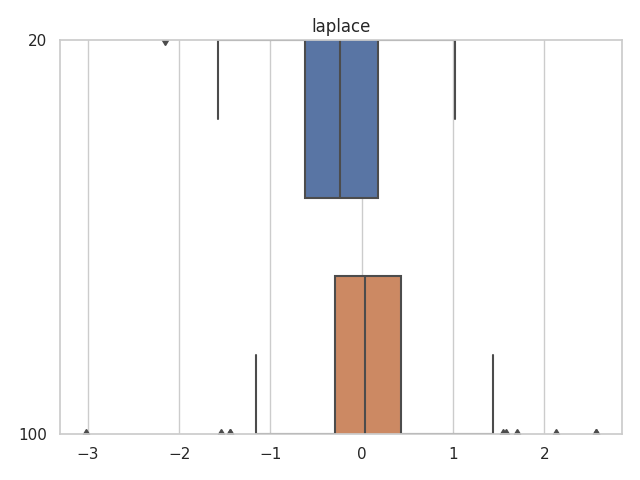
\includegraphics[width=\textwidth]{laplace.png} 
\end{figure}

\begin{figure}[H]
\caption{Boxplot стандартное распределение Коши }
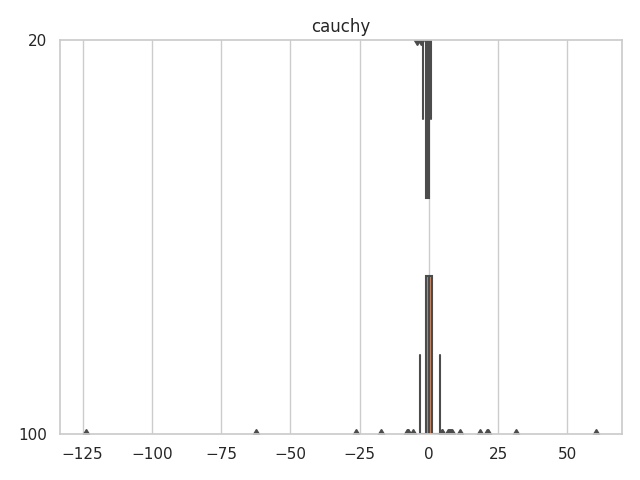
\includegraphics[width=\textwidth]{cauchy.png} 
\end{figure}

\begin{figure}[H]
\caption{Boxplot распределение Пуассона }
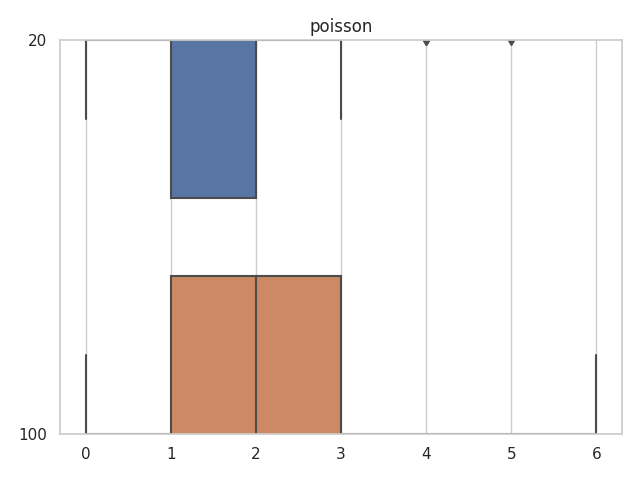
\includegraphics[width=\textwidth]{poisson.png} 
\end{figure}

\begin{figure}[H]
 \caption{Boxplot равномерное распределение }
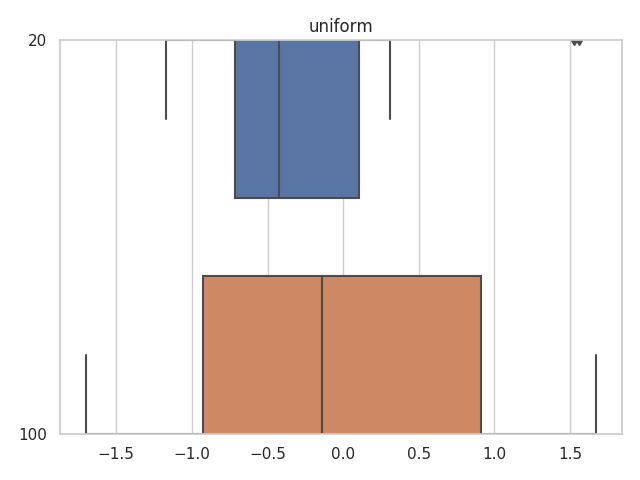
\includegraphics[width=\textwidth]{uniform.png}
\end{figure}

\begin{table}[H]
\caption{Зависимость выбросов от размера выборки}
\label{tab:my_label2}
\begin{center}
\vspace{5mm}
\begin{tabular}{|c|c|}
\hline
Выборка & Процент выбросов\\
\hline
normal&\\
\hline
n = 20    &3    \\
\hline
n = 100   &1    \\
\hline
cauchy&\\
\hline
n = 20    &15    \\
\hline
n = 100   &16    \\
\hline
laplace&\\
\hline
n = 20    &7    \\
\hline
n = 100   &6    \\
\hline
uniform &\\
\hline
n = 20    &0   \\
\hline
n = 100   &0    \\
\hline
poisson &
\\
\hline
n = 20    &2    \\
\hline
n = 100   &1    \\
\hline

\end{tabular}
\end{center}
\end{table}
\end{center}

\section{Выводы}
\par Экспериментально полученные проценты выбросок, близки к теоретическим
Можно вывести соотношение между процентами выбросов:

\begin{equation}
uniform<normal<poisson<laplace<cauchy
\end{equation}

\par По полученным данным видно, что наименьший процент выбросов у равномерного распределения, а наибольший процент выбросов у распределения Коши

\section{Приложения}

Исходники: \url{https://github.com/LanskovNV/math_statistics/tree/master/lab_3}

\begin{thebibliography}{}
    \bibitem{med}  
    Выборочная медиана  -  http://femto.com.ua/articles/part\_1/2194.html
    
    \bibitem{quart}  
    Квартили -  https://studfiles.net/preview/2438125/page:13/
    
    \bibitem{sas} 
    Боксплот - https://en.wikipedia.org/wiki/Box\_plot
    
    \bibitem{numpy}  
    Модуль numpy  -  https://physics.susu.ru/vorontsov/language/numpy.html
    
    \bibitem{plotlib} 
    Модуль matplotlib - https://matplotlib.org/users/index.html
    
 
\end{thebibliography}

\end{document}
